\documentclass[tikz,border=18pt]{standalone}
\usepackage{amsmath,amssymb}
\usetikzlibrary{positioning,calc}

\begin{document}
	
	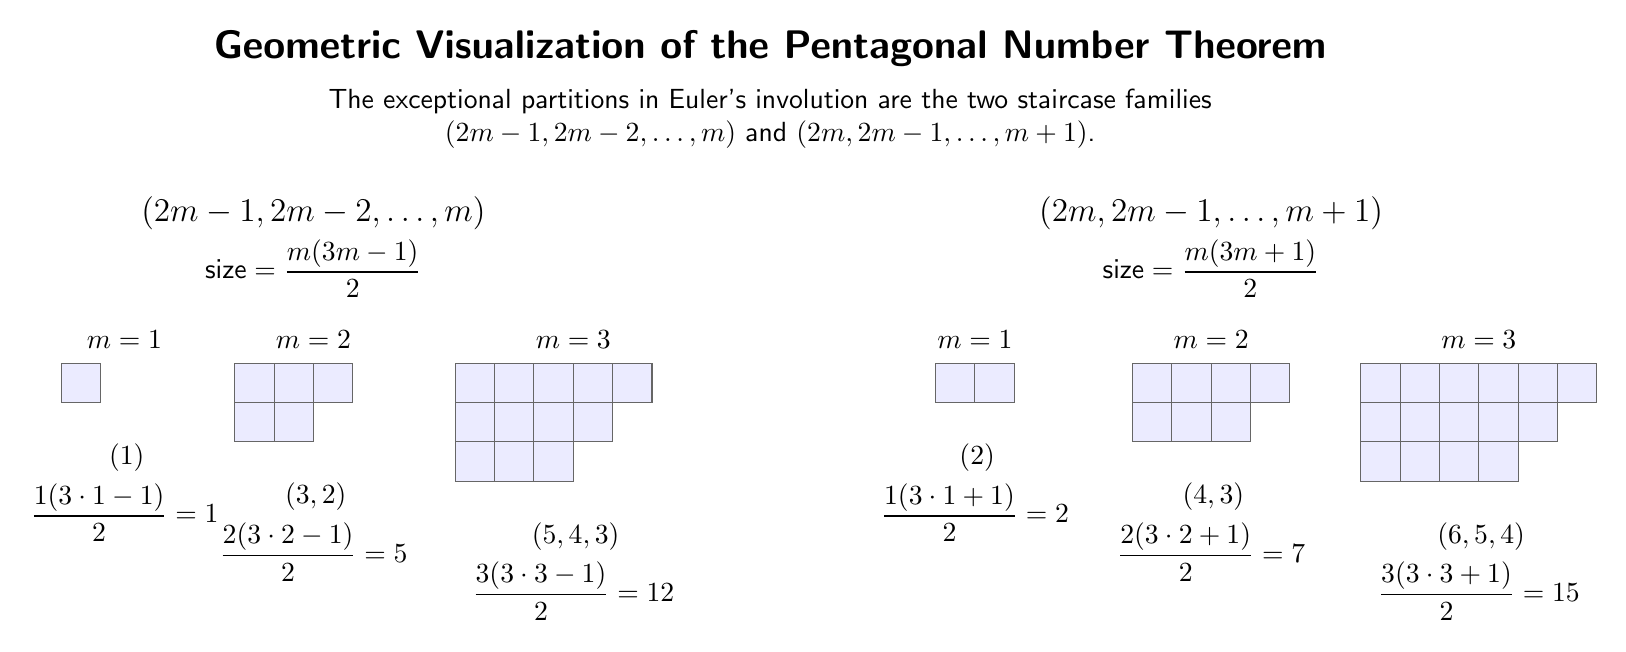
\begin{tikzpicture}[
		box/.style={draw=black!60, fill=blue!8, minimum size=5mm},
		title/.style={font=\sffamily\bfseries\Large},
		label/.style={font=\sffamily\large},
		note/.style={font=\sffamily\normalsize},
		every node/.style={inner sep=1pt}
		]
		
		% -------------------------------------------------
		% Title
		% -------------------------------------------------
		\node[title] at (9,9.8) {Geometric Visualization of the Pentagonal Number Theorem};
		
		\node[note, align=center] at (9,8.9) {
			The exceptional partitions in Euler's involution are the two staircase families\\
			$\displaystyle (2m-1,2m-2,\dots,m)$ and $\displaystyle (2m,2m-1,\dots,m+1)$.
		};
		
		% -------------------------------------------------
		% First family: m = 1,2,3
		% -------------------------------------------------
		\node[label] at (3.2,7.7) {$\left(2m-1,2m-2,\dots,m\right)$};
		\node[note] at (3.2,7.0) {$\displaystyle \text{size}=\frac{m(3m-1)}2$};
		
		% m=1
		\node[note] at (0.8,6.1) {$m=1$};
		\foreach \x in {0}
		\draw[box] (\x,5.3) rectangle ++(0.5,0.5);
		\node[note] at (0.8,4.6) {$\,(1)$};
		\node[note] at (0.8,3.9) {$\displaystyle \frac{1(3\cdot1-1)}2=1$};
		
		% m=2
		\node[note] at (3.2,6.1) {$m=2$};
		\foreach \x in {0,1,2}
		\draw[box] (2.2+\x*0.5,5.3) rectangle ++(0.5,0.5);
		\foreach \x in {0,1}
		\draw[box] (2.2+\x*0.5,4.8) rectangle ++(0.5,0.5);
		\node[note] at (3.2,4.1) {$\,(3,2)$};
		\node[note] at (3.2,3.4) {$\displaystyle \frac{2(3\cdot2-1)}2=5$};
		
		% m=3
		\node[note] at (6.5,6.1) {$m=3$};
		\foreach \x in {0,1,2,3,4}
		\draw[box] (5.0+\x*0.5,5.3) rectangle ++(0.5,0.5);
		\foreach \x in {0,1,2,3}
		\draw[box] (5.0+\x*0.5,4.8) rectangle ++(0.5,0.5);
		\foreach \x in {0,1,2}
		\draw[box] (5.0+\x*0.5,4.3) rectangle ++(0.5,0.5);
		\node[note] at (6.5,3.6) {$\,(5,4,3)$};
		\node[note] at (6.5,2.9) {$\displaystyle \frac{3(3\cdot3-1)}2=12$};
		
		% -------------------------------------------------
		% Second family: m = 1,2,3
		% -------------------------------------------------
		\node[label] at (14.6,7.7) {$\left(2m,2m-1,\dots,m+1\right)$};
		\node[note] at (14.6,7.0) {$\displaystyle \text{size}=\frac{m(3m+1)}2$};
		
		% m=1
		\node[note] at (11.6,6.1) {$m=1$};
		\foreach \x in {0,1}
		\draw[box] (11.1+\x*0.5,5.3) rectangle ++(0.5,0.5);
		\node[note] at (11.6,4.6) {$\,(2)$};
		\node[note] at (11.6,3.9) {$\displaystyle \frac{1(3\cdot1+1)}2=2$};
		
		% m=2
		\node[note] at (14.6,6.1) {$m=2$};
		\foreach \x in {0,1,2,3}
		\draw[box] (13.6+\x*0.5,5.3) rectangle ++(0.5,0.5);
		\foreach \x in {0,1,2}
		\draw[box] (13.6+\x*0.5,4.8) rectangle ++(0.5,0.5);
		\node[note] at (14.6,4.1) {$\,(4,3)$};
		\node[note] at (14.6,3.4) {$\displaystyle \frac{2(3\cdot2+1)}2=7$};
		
		% m=3
		\node[note] at (18.0,6.1) {$m=3$};
		\foreach \x in {0,1,2,3,4,5}
		\draw[box] (16.5+\x*0.5,5.3) rectangle ++(0.5,0.5);
		\foreach \x in {0,1,2,3,4}
		\draw[box] (16.5+\x*0.5,4.8) rectangle ++(0.5,0.5);
		\foreach \x in {0,1,2,3}
		\draw[box] (16.5+\x*0.5,4.3) rectangle ++(0.5,0.5);
		\node[note] at (18.0,3.6) {$\,(6,5,4)$};
		\node[note] at (18.0,2.9) {$\displaystyle \frac{3(3\cdot3+1)}2=15$};
		
%		% -------------------------------------------------
%		% Bottom summary
%		% -------------------------------------------------
%		\node[draw=black!50, fill=gray!8, rounded corners=3pt, align=center, text width=16cm] at (9,0.9) {
%			\textbf{Why this visualizes the theorem:}\\[1mm]
%			In Euler's sign-reversing involution on partitions into distinct parts, almost all Ferrers diagrams cancel in pairs.\\
%			The only unpaired diagrams are exactly these two staircase families, whose sizes are
%			\[
%			1,2,5,7,12,15,22,26,\dots
%			\]
%			that is,
%			\[
%			\frac{m(3m-1)}2 \quad\text{and}\quad \frac{m(3m+1)}2.
%			\]
%			These are the generalized pentagonal numbers appearing in
%			\[
%			\prod_{n\ge1}(1-q^n)=1+\sum_{m\ge1}(-1)^m\!\left(q^{m(3m-1)/2}+q^{m(3m+1)/2}\right).
%			\]
%		};
		
	\end{tikzpicture}
	
\end{document}